\documentclass[
11pt, % The default document font size, options: 10pt, 11pt, 12pt
%codirector, % Uncomment to add a codirector to the title page
]{charter} 




% El títulos de la memoria, se usa en la carátula y se puede usar el cualquier lugar del documento con el comando \ttitle
\titulo{Desarrollo de un dispositivo embebido localizador y botón antipánico} 

% Nombre del posgrado, se usa en la carátula y se puede usar el cualquier lugar del documento con el comando \degreename
% \posgrado{Carrera de Especialización en Sistemas Embebidos} 
\posgrado{Carrera de Especialización en Internet de las Cosas} 
%\posgrado{Carrera de Especialización en Intelegencia Artificial}
%\posgrado{Maestría en Sistemas Embebidos} 
%\posgrado{Maestría en Internet de las cosas}

% Tu nombre, se puede usar el cualquier lugar del documento con el comando \authorname
\autor{Ing. Erik Hromek} 

% El nombre del director y co-director, se puede usar el cualquier lugar del documento con el comando \supname y \cosupname y \pertesupname y \pertecosupname
\director{Mg. Ing. Lucas Dórdolo}
\pertenenciaDirector{FIUBA} 
% FIXME:NO IMPLEMENTADO EL CODIRECTOR ni su pertenencia
%\codirector{Por definir} % para que aparezca en la portada se debe descomentar la opción codirector en el documentclass
%\pertenenciaCoDirector{Por definir}

% Nombre del cliente, quien va a aprobar los resultados del proyecto, se puede usar con el comando \clientename y \empclientename
\cliente{???}
\empresaCliente{???}

% Nombre y pertenencia de los jurados, se pueden usar el cualquier lugar del documento con el comando \jurunoname, \jurdosname y \jurtresname y \perteunoname, \pertedosname y \pertetresname.
%\juradoUno{Nombre y Apellido (1)}
%\pertenenciaJurUno{pertenencia (1)} 
%\juradoDos{Nombre y Apellido (2)}
%\pertenenciaJurDos{pertenencia (2)}
%\juradoTres{Nombre y Apellido (3)}
%\pertenenciaJurTres{pertenencia (3)}
 
\fechaINICIO{20 de junio de 2023}		%Fecha de inicio de la cursada de GdP \fechaInicioName
\fechaFINALPlan{8 de julio de 2023} 	%Fecha de final de cursada de GdP
\fechaFINALTrabajo{???}	%Fecha de defensa pública del trabajo final


\begin{document}

\maketitle
\thispagestyle{empty}
\pagebreak


\thispagestyle{empty}
{\setlength{\parskip}{0pt}
\tableofcontents{}
}
\pagebreak


\section*{Registros de cambios}
\label{sec:registro}


\begin{table}[ht]
\label{tab:registro}
\centering
\begin{tabularx}{\linewidth}{@{}|c|X|c|@{}}
\hline
\rowcolor[HTML]{C0C0C0} 
Revisión & \multicolumn{1}{c|}{\cellcolor[HTML]{C0C0C0}Detalles de los cambios realizados} & Fecha      \\ \hline
0      & Creación del documento                                 &\fechaInicioName \\ \hline
1      & Se completa hasta el punto 5 inclusive                 & 04/07/2023 \\ \hline
2          & Se aplican correcciones hasta el punto 5 inclusive                  & 9/07/2023 \\ \hline
3          & Se completa hasta el punto 9 inclusive                 & 11/07/2023 \\ \hline

%2      & Se completa hasta el punto 7 inclusive
%		  Se puede agregar algo más \newline
%		  En distintas líneas \newline
%		  Así                                                    & dd/mm/aaaa \\ \hline
%3      & Se completa hasta el punto 11 inclusive                & dd/mm/aaaa \\ \hline
%4      & Se completa el plan	                                 & dd/mm/aaaa \\ \hline
\end{tabularx}
\end{table}

\pagebreak



\section*{Acta de constitución del proyecto}
\label{sec:acta}

\begin{flushright}
Buenos Aires, \fechaInicioName
\end{flushright}

\vspace{2cm}

Por medio de la presente se acuerda con el Ing. \authorname\hspace{1px} que su Trabajo Final de la \degreename\hspace{1px} se titulará ``\ttitle'', consistirá esencialmente en la implementación de un prototipo de un botón antipánico y localizador, y tendrá un presupuesto preliminar estimado de \textcolor{red}{600} h de trabajo y \textcolor{red}{\$XXX}, con fecha de inicio el \fechaInicioName\hspace{1px} y fecha de presentación pública \fechaFinalName.

Se adjunta a esta acta la planificación inicial.

\vfill

% Esta parte se construye sola con la información que hayan cargado en el preámbulo del documento y no debe modificarla
\begin{table}[ht]
\centering
\begin{tabular}{ccc}
\begin{tabular}[c]{@{}c@{}}Dr. Ing. Ariel Lutenberg \\ Director posgrado FIUBA\end{tabular} & \hspace{2cm} & \begin{tabular}[c]{@{}c@{}}\clientename \\ \empclientename \end{tabular} \vspace{2.5cm} \\ 
\multicolumn{3}{c}{\begin{tabular}[c]{@{}c@{}} \supname \\ Director del Trabajo Final\end{tabular}} \vspace{2.5cm} \\
%\begin{tabular}[c]{@{}c@{}}\jurunoname \\ Jurado del Trabajo Final\end{tabular}     &  & \begin{tabular}[c]{@{}c@{}}\jurdosname\\ Jurado del Trabajo Final\end{tabular}  \vspace{2.5cm}  \\
%\multicolumn{3}{c}{\begin{tabular}[c]{@{}c@{}} \jurtresname\\ Jurado del Trabajo Final\end{tabular}} \vspace{.5cm}                                                                     
\end{tabular}
\end{table}




\section{1. Descripción técnica-conceptual del proyecto a realizar}
\label{sec:descripcion}


El proyecto consiste, en primer lugar, en la investigación y el desarrollo de un prototipo de un dispositivo localizador que funcione como botón antipánico. En segundo lugar, incluye la implementación de una prueba de concepto de una aplicación web que permita recibir y registrar las activaciones del botón antipánico.

Resulta importante realizar una introducción al contexto en el cual se desarrolla este proyecto. Esto permitirá entender los motivos originales del autor, desafíos técnicos del proyecto y las consideraciones/restricciones de este.
El autor tiene experiencia en la adquisición, configuración, implementación y soporte de botones antipánico disponibles en el mercado. Se observa que varios de estos presentan los siguientes inconvenientes:
\begin{itemize}
	\item Especificaciones de hardware obsoletas.
	\item Documentación escasa, desactualizada o incluso incorrecta en algunos casos.
	\item Poca fiabilidad de dispositivo (dificultad para configurarlos, mala señal, desconfianza al momento de utilizarlo).
	\item Inconsistencias entre dispositivos idénticos.
	\item Poca duración de batería (desde aproximadamente 24 horas hasta 3 o 4 días como máximo, cuando lo deseable para el beneficiario final del botón es de al menos 5 o 6 días).
	\item Precio exageradamente elevado y muchas dificultades para adquirirlos mediante proveedores.
	\item Nulas características de seguridad.
\end{itemize}

Se ha investigado y revisado diferentes alternativas en el mercado, así como también se ha trabajado con dispositivos utilizados por sistemas de la competencia llegando a conclusiones similares: no se encuentran dispositivos aceptables cuyo costo sea accesible. 
Por ello, uno de los principales motivos del proyecto es lograr construir un dispositivo que permita validar las elecciones tecnológicas y tener una fiabilidad superior, en comparación con los dispositivos disponibles en el mercado.

Descrito el contexto en el cual se encuentra el proyecto a desarrollar, es de interés realizar una breve introducción de los componentes involucrados. En la figura 1 se observan los componentes con los que contará, como mínimo, el prototipo a construir:
\begin{itemize}
	\item Microcontrolador: permitirá el desarrollo del sistema embebido.
	\item Módulo de telefonía móvil: permitirá conectividad y comunicación mediante SMS y redes IP.
	\item Batería: servirá para el uso del dispositivo de forma autónoma.
	\item Módulo GNSS (\textit{Global Navigation Satellite System}): obtendrá la ubicación geográfica del usuario del botón.
	\item Almacenamiento: permitirá el guardado de la configuración y parámetros del dispositivo.
	\item Activador: actuador físico que disparará una alerta y notificar al sistema web.
\end{itemize}

Adicionalmente, se encuentran algunos componentes web a incorporar en el marco del proyecto:

\begin{itemize}
	\item API receptora de SMS: permitirá la recepción de mensajes del texto del dispositivo y enviarlos a otro sistema.
	\item Aplicación web de seguimiento: aplicación compuesta por un \textit{backend} y un \textit{frontend} que posibilitará registrar y almacenar las alertas.
	\item Base de datos: funcionará como almacenamiento persistente de la aplicación web anterior.
\end{itemize}

Estos componentes se utilizarán a modo de prueba de concepto para probar el correcto funcionamiento del prototipo de botón. También funcionarán como caso de uso para integrar este dispositivo a cualquier plataforma web de similares características.

\begin{figure}[htpb]
\centering 
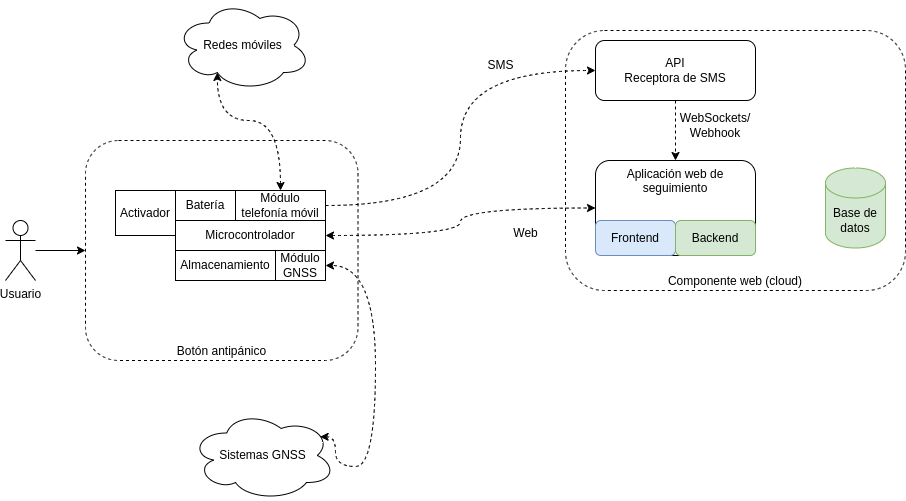
\includegraphics[width=1\textwidth]{./Figuras/diagBloques.png}
\caption{Diagrama en bloques del dispositivo y los componentes web a desarrollar.}
\label{fig:diagBloques}
\end{figure}

\section{2. Identificación y análisis de los interesados}
\label{sec:interesados}

\begin{table}[ht]
%\caption{Identificación de los interesados}
%\label{tab:interesados}
\begin{tabularx}{\linewidth}{@{}|l|X|X|l|@{}}
\hline
\rowcolor[HTML]{C0C0C0} 
Rol           & Nombre y Apellido & Organización 	& Puesto 	\\ \hline
Responsable   & \authorname       & FIUBA        	& Alumno 	\\ \hline
Orientador    & \supname	      & \pertesupname 	& Director Trabajo final \\ \hline
Usuario Final    & Ciudadano & - 	& - \\ \hline
\end{tabularx}
\end{table}


\begin{itemize}
	\item Responsable: principal interesado en la implementación exitosa del dispositivo, posee interés en continuar con el trabajo en futuras etapas.
	\item Orientador: el directo posee experiencia dirigiendo aplicaciones con características similares, pero no posee una gran disponibilidad para colaborar; debe acudirse a él solamente con cuestiones muy focalizadas
\end{itemize}


\section{3. Propósito del proyecto}
\label{sec:proposito}

El propósito de este proyecto es validar la idea de que es posible implementar, al menos de forma inicial, un dispositivo que funcione como botón antipánico y localizador. Se busca lograr que este dispositivo permita notificar la ubicación del usuario final al momento de ser activado via SMS o web y que además trabaje de forma autónoma con una batería.

\section{4. Alcance del proyecto}
\label{sec:alcance}

Para la realización de este proyecto se llevará a cabo:
\begin{itemize}
	\item una investigación preliminar en relación a los componentes a utilizar,
	\item la implementación del hardware del botón antipánico,
	\item el desarrollo del firmware o software para controlar el dispositivo y
	\item el desarrollo de una plataforma web para recibir las activaciones del botón antipánico.
\end{itemize}


La implementación del dispositivo incluirá:
\begin{itemize}
	\item conectividad mediante redes móviles,
	\item el uso de un módulo de posicionamiento satelital para tomar la ubicación actual de la persona y
	\item un mecanismo de configuración/parametrización del dispositivo que sea persistente.
\end{itemize}
Además, contará con alimentación mediante una batería de prestaciones acordes al tamaño del dispositivo y se realizará una investigación acerca del consumo energético de este.

El desarrollo de la plataforma web incluirá la implementación de un servicio online que permita recepcionar mensajes de texto desde teléfonos de Argentina, el registro y visualización de las alertas, a modo de prueba de concepto.

Este proyecto no incluirá:
\begin{itemize}
	\item Aplicación web productiva para gestionar las activaciones del botón antipánico. Por productiva se refiere a que pueda ser ofrecida al mercado o utilizable por usuarios encargados del monitoreo.
	\item Desarrollo de un dispositivo listo para ser lanzado al mercado, es decir que no sea un prototipo.
	\item Desarrollo de un contenedor para el dispositivo.
\end{itemize}

\section{5. Supuestos del proyecto}
\label{sec:supuestos}

\begin{itemize}
	\item Todos los componentes de hardware a utilizar serán definidos luego de una una investigación preliminar.
	\item Se intentará utilizar parte del material aprendido durante el curso de especialización relacionado a la programación de sistemas embebidos (bibliotecas, firmware, etc.).
	\item Se utilizará un microcontrolador que pueda ser adquirido a un costo relativamente bajo.
	\item Se contará con un chip de telefonía móvil para utilizar en el proyecto.
	\item Se adquirirán: un módulo de localización satelital, una batería compatible, un módulo de telefonía móvil y un pulsador que estén disponibles en el mercado local.
	\item Para recibir los SMS, se contratará un servicio web que permita recibir los mensajes y redireccionarlos a la aplicación web.

\end{itemize}

\section{6. Requerimientos}
\label{sec:requerimientos}

Los requerimientos se listan agrupados por afinidad:

\begin{enumerate}
\item Grupo de requerimientos del dispositivo geolocalizador:
	\begin{enumerate}
	\item Contar una batería recargable que dure al menos 120 horas (5 días) y sea cargable mediante un cable \textit{Micro USB}.
	\item Contar con botones para encendido/apagado y activación de una alerta.
	\item Tener un indicador del estado del dispositivo: encendido/apagado, señal de telefonía móvil, señal de GPS y nivel de batería.
	\item Contar con conectividad a la red de telefonía móvil.
	\item Obtener períodicamente la ubicación actual del dispositivo y guardarla internamente.
	\item Permitir configurar un número de teléfono para enviar una alerta por mensaje de texto.
	\item Tener un mecanismo de notificación cuando se dispare una alerta, mediante vibración o sonido.
	\item Incluir la ubicación del dispositivo en el mensaje de alerta.
	\item Poder configurar un número de teléfono como administrador del dispositivo.
	\item Permitir configurar parámetros necesarios para el funcionamiento del dispositivo, por ejemplo datos de la red de telefonía móvil.
	\item Contar con almacenamiento persistente para la configuración.
	\end{enumerate}
\item Grupo de requerimientos asociados al sistema web de gestión de dispositivos y alertas:
	\begin{enumerate}
	\item Recibir y almacenar las alertas enviadas a un número de teléfono designado.
	\item Permitir crear usuarios administradores.
	\item Contar con un acceso web para poder cargar nuevos dispositivos y visualizar alertas.
	\item Contar con una sección para visualizar y exportar el historial de alertas de un dispositivo.
	\item Impedir que un dispositivo no habilitado envíe alertas al sistema.
	\item Debe poder ser desplegable en un entorno \textit{cloud} u \textit{on-premise}.
	\end{enumerate}
\item Grupo de requerimientos de documentación:
	\begin{enumerate}
	\item Incluir un \textit{datasheet} del dispositivo que permita la integración del dispositivo a otros sistemas web.
	\item Incorporar un manual de configuración del dispositivo.
	\item Contar con una licencia de código abierto para el dispositivo.
	\end{enumerate}
\end{enumerate}

\section{7. Historias de usuarios (\textit{Product backlog})}
\label{sec:backlog}

Respecto al peso, se asignarán los valores de acuerdo a una escala basada en la sucesión de Fibonacci, siendo 1 el valor más bajo y 21 el valor más alto, representando este número una tarea extremadamente compleja.

\begin{itemize}
	\item Como usuario del dispositivo deseo poder visualizar el estado de: el dispositivo, la batería, la señal de telefonía móvil y la señal de GPS. Valor: 13.
	\item Como usuario del dispositivo quiero que el dispositivo tenga un botón físico para prender y apagar el dispositivo. Valor: 5.
	\item Como usuario del dispositivo deseo poder disparar un alerta mediante un botón y recibir una notificación del dispositivo indicando que se disparó la alerta: Valor: 5.
	\item Como usuario del dispositivo deseo poder cargar el dispositivo con un cargador similar al de los teléfonos móviles para poder utilizarlo en cualquier lugar. Valor: 5.
	\item Como usuario administrador quiero poder configurar un teléfono asociado a un dispositivo para que reporte alertas hacia el número designado. Valor: 3.
	\item Como usuario administrador quiero poder recuperar la configuración actual del dispositivo para saber cómo está configurado actualmente. Valor: 3.
	\item Como usuario administrador quiero poder limitar quién puede configurar el dispositivo para que solamente yo pueda modificar su funcionamiento. Valor: 5.
	\item Como usuario administrador quiero poder ingresar a la plataforma web mediante un \textit{login} para hacer uso de esta. Valor: 5.
	\item Como usuario administrador quiero poder crear nuevos usuarios para que tengan acceso a la plataforma web. Valor: 3.
	\item Como usuario administrador quiero poder dar de alta dispositivos para utilizar como botones antipánico. Valor: 5.
	\item Como usuario administrador quiero poder recibir, visualizar y almacenar en tiempo real las alertas recibidas en el sistema web para gestionarlas. Valor: 13.
	\item Como usuario administrador quiero poder visualizar y exportar un reporte de alertas de un dispositivo para tener la información por fuera del sistema web. Valor: 8.
	\item Como usuario administrador quiero contar con un manual de los dispositivos para poder configurarlos. Valor: 3.

\end{itemize}


\section{8. Entregables principales del proyecto}
\label{sec:entregables}


Los entregables del proyecto son:

\begin{itemize}
	\item Prototipo de dispositivo geolocalizador
	\item Aplicación web desplegada en un entorno \textit{cloud}
	\item Código fuente del firmware del dispositivo
	\item Código fuente de la aplicación web
	\item Documentación asociada a la aplicación web
	\item Manual del dispositivo
	\item Informe final
\end{itemize}

\section{9. Desglose del trabajo en tareas}
\label{sec:wbs}


\begin{enumerate}
\item Planificación del proyecto (44 hs)
	\begin{enumerate}
	\item Definición de requerimientos (10 hs)
	\item Armado de documentación (32 hs)
	\item Revisión de requerimientos con el director (2 hs)
	\end{enumerate}
\item Investigación previa (60 hs)
	\begin{enumerate}
	\item Investigación de microcontrolador y plataforma a usar (8 hs)
	\item Investigación de módulos y sensores a adquirir (12 hs)
	\item Análisis del consumo de energía del dispositivo y los módulos (8 hs)
	\item Investigación y comparación de proveedores \textit{cloud} (8 hs)
	\item Análisis de tecnologías web (8 hs)
	\item Investigación de servicios para interfaz web receptora de SMS (12 hs)
	\item Definición de entornos de desarrollo para la programación embebida y web (4 hs)
	\end{enumerate}
\item Desarrollo e implementación de dispositivo embebido (134 hs)
	\begin{enumerate}
	\item \textit{Setup} inicial del firmware (6 hs)
	\item Realizar diagrama esquemático del dispositivo y sus módulos (8 hs)
	\item Realizar pruebas iniciales de conexión del dispositivo y sus módulos (8 hs)
	\item Desarrollo del sistema asociado al módulo de telefonía móvil (16 hs)
	\item Desarrollo del sistema asociado al módulo de localización satelital (12 hs)
	\item Desarrollo del sistema asociado al módulo de configuración y almacenamiento de parámetros (16 hs)
	\item Desarrollo del sistema asociado a la gestión del estado del dispositivo (20 hs)
	\item Desarrollo del sistema asociado al módulo de alertas (12 hs)
	\item Desarrollo del sistema asociado al manejo de batería y energía del dispositivo (16 hs)
	\item Integración entre todos los módulos al sistema operativo de tiempo real (20 hs)
	\end{enumerate}
\item Desarrollo y despliegue de sistema web (206 hs)
	\begin{enumerate}
	\item Armado de modelo de datos (12 hs)
	\item Armado de maquetas funcionales para interfaz de usuario (8 hs)
	\item \textit{Setup} inicial del \textit{backend} (4 hs)
	\item Desarrollo de módulo de gestión de usuarios (16 hs)
	\item Desarrollo de módulo de gestión de dispositivos (16 hs)
	\item Implementación de módulo de recepción de alertas (20 hs)
	\item Desarrollo de módulo de gestión de alertas (20 hs)
	\item Implementación de pruebas unitarias generales del \textit{backend} (20 hs)
	\item \textit{Setup} inicial del \textit{frontend} (2 hs)
	\item Desarrollo de interfaces de usuario de administración (25 hs)
	\item Desarrollo de interfaz de usuario para gestión de alertas (40 hs)
	\item Integración al \textit{backend} y pruebas de interfaces de usuario (20 hs)
	\item Despliegue de sistema web (6 hs)
	\end{enumerate}
\item Pruebas de funcionamiento del sistema (46 hs)
	\begin{enumerate}
	\item Pruebas del dispositivo (30 hs)
	    \begin{enumerate}
	    \item Pruebas de funcionamiento de la conexión del dispositivo a la red de telefonía móvil (4 hs)
	    \item Pruebas de funcionamiento de la localización satelital del dispositivo (4 hs)
	    \item Pruebas de funcionamiento del dispositivo con los indicadores de estado (4 hs)
	    \item Pruebas de funcionamiento de las alertas del dispositivo (4 hs)
	    \item Pruebas de funcionamiento de la configuración persistente del dispositivo (4 hs)	
	    \item Pruebas de funcionamiento de la duración de la batería (8 hs)
	    \item Pruebas de funcionamiento del dispositivo con el actuador de encedido (2 hs)
	    \end{enumerate}
	\item Pruebas del sistema web (28 hs)
	    \begin{enumerate}
	    \item Pruebas de funcionamiento de creación y edición de usuarios (6 hs)
	    \item Pruebas de funcionamiento de creación y edición de dispositivos (6 hs)
	    \item Pruebas de funcionamiento de módulo de gestión de alertas (8 hs)
	    \item Pruebas de circuito completo del dispositivo y la plataforma (8 hs)
	    \end{enumerate}
	\end{enumerate}
\item Armado de documentación y manuales (36 hs)
	\begin{enumerate}
	\item Armado de manual del dispositivo (20 hs)
	\item Armado de documentación del sistema web (16 hs)
	\end{enumerate}
\item Elaboración de documentación del proyecto (60 hs)
	\begin{enumerate}
	\item Elaboración de memoria técnica del proyecto (40 hs)
	\item Elaboración de presentación del proyecto (20 hs)
	\end{enumerate}
\end{enumerate}

Cantidad total de horas estimadas: 598 hs

\section{10. Diagrama de Activity On Node}
\label{sec:AoN}

\begin{consigna}{red}
Armar el AoN a partir del WBS definido en la etapa anterior. 

%La figura \ref{fig:AoN} fue elaborada con el paquete latex tikz y pueden consultar la siguiente referencia \textit{online}:

%\url{https://www.overleaf.com/learn/latex/LaTeX_Graphics_using_TikZ:_A_Tutorial_for_Beginners_(Part_3)\%E2\%80\%94Creating_Flowcharts}

\end{consigna}

\begin{figure}[htpb]
\centering 
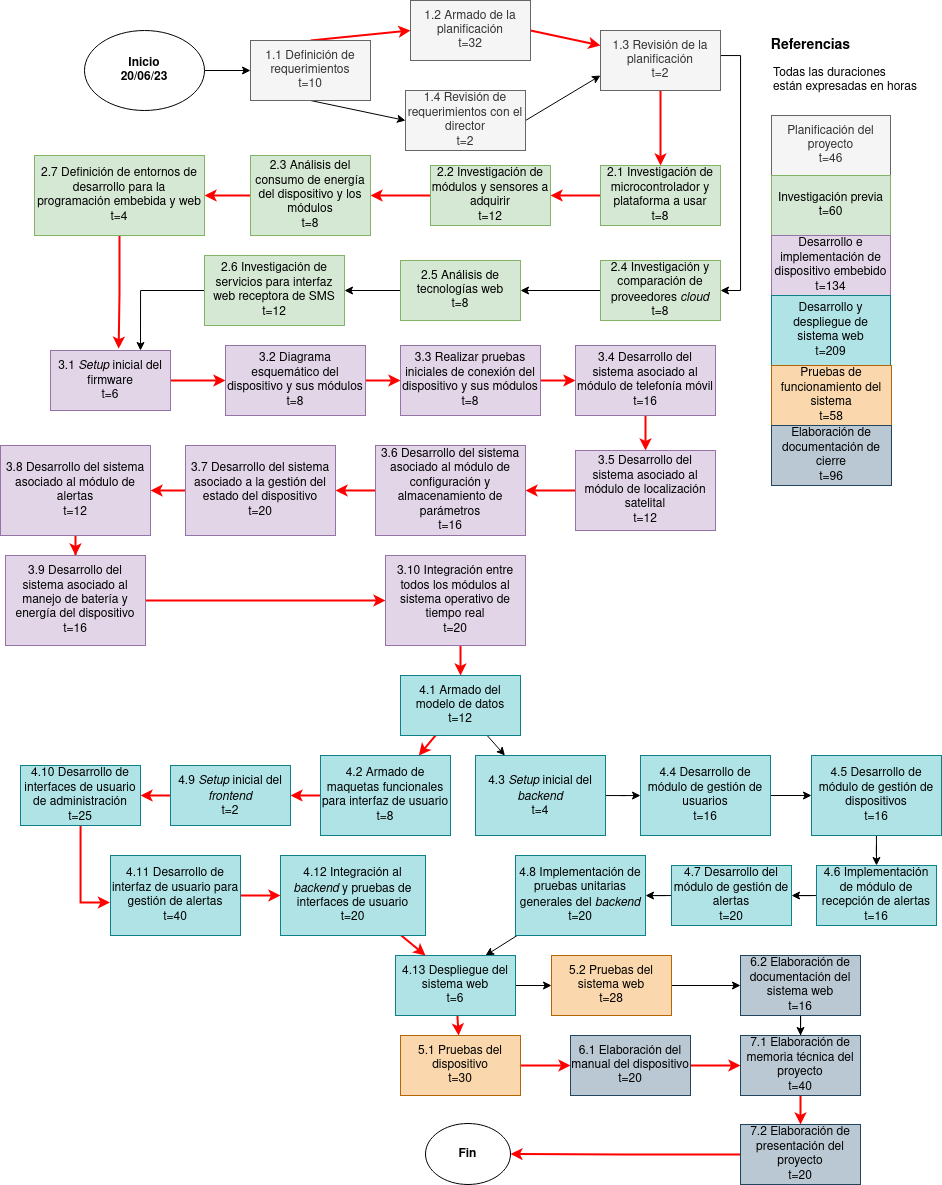
\includegraphics[width=.8\textwidth]{./Figuras/AoN.png}
\caption{Diagrama de \textit{Activity on Node}.}
\label{fig:AoN}
\end{figure}

Indicar claramente en qué unidades están expresados los tiempos.
De ser necesario indicar los caminos semicríticos y analizar sus tiempos mediante un cuadro.
Es recomendable usar colores y un cuadro indicativo describiendo qué representa cada color, como se muestra en el siguiente ejemplo:



\section{11. Diagrama de Gantt}
\label{sec:gantt}

\begin{consigna}{red}

Existen muchos programas y recursos \textit{online} para hacer diagramas de Gantt, entre los cuales destacamos:

\begin{itemize}
\item Planner
\item GanttProject
\item Trello + \textit{plugins}. En el siguiente link hay un tutorial oficial: \\ \url{https://blog.trello.com/es/diagrama-de-gantt-de-un-proyecto}
\item Creately, herramienta online colaborativa. \\\url{https://creately.com/diagram/example/ieb3p3ml/LaTeX}
\item Se puede hacer en latex con el paquete \textit{pgfgantt}\\ \url{http://ctan.dcc.uchile.cl/graphics/pgf/contrib/pgfgantt/pgfgantt.pdf}
\end{itemize}

Pegar acá una captura de pantalla del diagrama de Gantt, cuidando que la letra sea suficientemente grande como para ser legible. 
Si el diagrama queda demasiado ancho, se puede pegar primero la ``tabla'' del Gantt y luego pegar la parte del diagrama de barras del diagrama de Gantt.

Configurar el software para que en la parte de la tabla muestre los códigos del EDT (WBS).\\
Configurar el software para que al lado de cada barra muestre el nombre de cada tarea.\\
Revisar que la fecha de finalización coincida con lo indicado en el Acta Constitutiva.

En la figura \ref{fig:gantt}, se muestra un ejemplo de diagrama de Gantt realizado con el paquete de \textit{pgfgantt}. En la plantilla pueden ver el código que lo genera y usarlo de base para construir el propio.

\begin{figure}[htbp]
\begin{center}
\begin{ganttchart}{1}{12}
  \gantttitle{2020}{12} \\
  \gantttitlelist{1,...,12}{1} \\
  \ganttgroup{Group 1}{1}{7} \\
  \ganttbar{Task 1}{1}{2} \\
  \ganttlinkedbar{Task 2}{3}{7} \ganttnewline
  \ganttmilestone{Milestone o hito}{7} \ganttnewline
  \ganttbar{Final Task}{8}{12}
  \ganttlink{elem2}{elem3}
  \ganttlink{elem3}{elem4}
\end{ganttchart}
\end{center}
\caption{Diagrama de Gantt de ejemplo}
\label{fig:gantt}
\end{figure}


\begin{landscape}
\begin{figure}[htpb]
\centering 
\includegraphics[height=.85\textheight]{./Figuras/Gantt-2.png}
\caption{Ejemplo de diagrama de Gantt rotado}
\label{fig:diagGantt}
\end{figure}

\end{landscape}

\end{consigna}


\section{12. Presupuesto detallado del proyecto}
\label{sec:presupuesto}

\begin{consigna}{red}
Si el proyecto es complejo entonces separarlo en partes:
\begin{itemize}
	\item Un total global, indicando el subtotal acumulado por cada una de las áreas.
	\item El desglose detallado del subtotal de cada una de las áreas.
\end{itemize}

IMPORTANTE: No olvidarse de considerar los COSTOS INDIRECTOS.

\end{consigna}

\begin{table}[htpb]
\centering
\begin{tabularx}{\linewidth}{@{}|X|c|r|r|@{}}
\hline
\rowcolor[HTML]{C0C0C0} 
\multicolumn{4}{|c|}{\cellcolor[HTML]{C0C0C0}COSTOS DIRECTOS} \\ \hline
\rowcolor[HTML]{C0C0C0} 
Descripción &
  \multicolumn{1}{c|}{\cellcolor[HTML]{C0C0C0}Cantidad} &
  \multicolumn{1}{c|}{\cellcolor[HTML]{C0C0C0}Valor unitario} &
  \multicolumn{1}{c|}{\cellcolor[HTML]{C0C0C0}Valor total} \\ \hline
 &
  \multicolumn{1}{c|}{} &
  \multicolumn{1}{c|}{} &
  \multicolumn{1}{c|}{} \\ \hline
 &
  \multicolumn{1}{c|}{} &
  \multicolumn{1}{c|}{} &
  \multicolumn{1}{c|}{} \\ \hline
\multicolumn{1}{|l|}{} &
   &
   &
   \\ \hline
\multicolumn{1}{|l|}{} &
   &
   &
   \\ \hline
\multicolumn{3}{|c|}{SUBTOTAL} &
  \multicolumn{1}{c|}{} \\ \hline
\rowcolor[HTML]{C0C0C0} 
\multicolumn{4}{|c|}{\cellcolor[HTML]{C0C0C0}COSTOS INDIRECTOS} \\ \hline
\rowcolor[HTML]{C0C0C0} 
Descripción &
  \multicolumn{1}{c|}{\cellcolor[HTML]{C0C0C0}Cantidad} &
  \multicolumn{1}{c|}{\cellcolor[HTML]{C0C0C0}Valor unitario} &
  \multicolumn{1}{c|}{\cellcolor[HTML]{C0C0C0}Valor total} \\ \hline
\multicolumn{1}{|l|}{} &
   &
   &
   \\ \hline
\multicolumn{1}{|l|}{} &
   &
   &
   \\ \hline
\multicolumn{1}{|l|}{} &
   &
   &
   \\ \hline
\multicolumn{3}{|c|}{SUBTOTAL} &
  \multicolumn{1}{c|}{} \\ \hline
\rowcolor[HTML]{C0C0C0}
\multicolumn{3}{|c|}{TOTAL} &
   \\ \hline
\end{tabularx}%
\end{table}


\section{13. Gestión de riesgos}
\label{sec:riesgos}

\begin{consigna}{red}
a) Identificación de los riesgos (al menos cinco) y estimación de sus consecuencias:
 
Riesgo 1: detallar el riesgo (riesgo es algo que si ocurre altera los planes previstos de forma negativa)
\begin{itemize}
	\item Severidad (S): mientras más severo, más alto es el número (usar números del 1 al 10).\\
	Justificar el motivo por el cual se asigna determinado número de severidad (S).
	\item Probabilidad de ocurrencia (O): mientras más probable, más alto es el número (usar del 1 al 10).\\
	Justificar el motivo por el cual se asigna determinado número de (O). 
\end{itemize}   

Riesgo 2:
\begin{itemize}
	\item Severidad (S): 
	\item Ocurrencia (O):
\end{itemize}

Riesgo 3:
\begin{itemize}
	\item Severidad (S): 
	\item Ocurrencia (O):
\end{itemize}


b) Tabla de gestión de riesgos:      (El RPN se calcula como RPN=SxO)

\begin{table}[htpb]
\centering
\begin{tabularx}{\linewidth}{@{}|X|c|c|c|c|c|c|@{}}
\hline
\rowcolor[HTML]{C0C0C0} 
Riesgo & S & O & RPN & S* & O* & RPN* \\ \hline
       &   &   &     &    &    &      \\ \hline
       &   &   &     &    &    &      \\ \hline
       &   &   &     &    &    &      \\ \hline
       &   &   &     &    &    &      \\ \hline
       &   &   &     &    &    &      \\ \hline
\end{tabularx}%
\end{table}

Criterio adoptado: 
Se tomarán medidas de mitigación en los riesgos cuyos números de RPN sean mayores a...

Nota: los valores marcados con (*) en la tabla corresponden luego de haber aplicado la mitigación.

c) Plan de mitigación de los riesgos que originalmente excedían el RPN máximo establecido:
 
Riesgo 1: plan de mitigación (si por el RPN fuera necesario elaborar un plan de mitigación).
  Nueva asignación de S y O, con su respectiva justificación:
  - Severidad (S): mientras más severo, más alto es el número (usar números del 1 al 10).
          Justificar el motivo por el cual se asigna determinado número de severidad (S).
  - Probabilidad de ocurrencia (O): mientras más probable, más alto es el número (usar del 1 al 10).
          Justificar el motivo por el cual se asigna determinado número de (O).

Riesgo 2: plan de mitigación (si por el RPN fuera necesario elaborar un plan de mitigación).
 
Riesgo 3: plan de mitigación (si por el RPN fuera necesario elaborar un plan de mitigación).

\end{consigna}


\section{14. Gestión de la calidad}
\label{sec:calidad}

\begin{consigna}{red}
Elija al menos diez requerientos que a su criterio sean los más importantes/críticos/que aportan más valor y para cada uno de ellos indique las acciones de verificación y validación que permitan asegurar su cumplimiento.

\begin{itemize} 
\item Req \#1: copiar acá el requerimiento.

\begin{itemize}
	\item Verificación para confirmar si se cumplió con lo requerido antes de mostrar el sistema al cliente. Detallar 
	\item Validación con el cliente para confirmar que está de acuerdo en que se cumplió con lo requerido. Detallar  
\end{itemize}

\end{itemize}

Tener en cuenta que en este contexto se pueden mencionar simulaciones, cálculos, revisión de hojas de datos, consulta con expertos, mediciones, etc.  Las acciones de verificación suelen considerar al entregable como ``caja blanca'', es decir se conoce en profundidad su funcionamiento interno.  En cambio, las acciones de validación suelen considerar al entregable como ``caja negra'', es decir, que no se conocen los detalles de su funcionamiento interno.

\end{consigna}

\section{15. Procesos de cierre}    
\label{sec:cierre}

\begin{consigna}{red}
Establecer las pautas de trabajo para realizar una reunión final de evaluación del proyecto, tal que contemple las siguientes actividades:

\begin{itemize}
	\item Pautas de trabajo que se seguirán para analizar si se respetó el Plan de Proyecto original:
	 - Indicar quién se ocupará de hacer esto y cuál será el procedimiento a aplicar. 
	\item Identificación de las técnicas y procedimientos útiles e inútiles que se emplearon, y los problemas que surgieron y cómo se solucionaron:
	 - Indicar quién se ocupará de hacer esto y cuál será el procedimiento para dejar registro.
	\item Indicar quién organizará el acto de agradecimiento a todos los interesados, y en especial al equipo de trabajo y colaboradores:
	  - Indicar esto y quién financiará los gastos correspondientes.
\end{itemize}

\end{consigna}


\end{document}
